\label{chap:pt1_chapter5}
The original problem consists of determining, given the workpiece geometry, the available fixtures (possibly of different sizes), and the available worktable bars, a set of fixtures together with their positions, orientations, and types that maximize workpiece stability.

We first consider a simplified version of the problem, assuming that the workpiece does not contain areas to be extruded and neglecting fixture rotations. Under these assumptions, to ensure the feasibility of a layout the following constraints must be satisfied:
\begin{enumerate}
	\item the number of placed fixtures must not exceed their availability;
	\item fixtures must be positioned so as to satisfy the minimum safety distances;
	\item fixtures must lie within the boundaries of the workpiece and beneath its surface;
	\item fixtures must not overlap each other.
\end{enumerate}

We address this problem by proposing a CP model implemented in the MiniZinc language~\cite{nethercote2007minizinc}. The model is parametric with respect to the input data and solver-independent. Consequently, it can be solved using any solver that support MiniZinc, not only CP-based solver, but also alternatives such as Mixed-Integer Programming (MIP) and Constraint Logic Programming (CLP) solvers.

\section{Model formulation}
\label{sec:first_cp_model}
In this section we describe the CP model in terms of input parameters, variables, constraints, and objective function(s). 
The model is \emph{parametric} because it is defined in terms of its parameters: changing the input data does not affect the model itself.

\subsection{Parameters}
\label{sec:first_parameters}
The input parameters shaping a particular problem instance are:

\begin{itemize}
	\item the width $\wtab$ and height $\htab$ of the machine worktable;
	\item the minimum horizontal distance $\wmin$ between two fixtures placed on different bars;
	\item the number $\ntypes$ of different fixture types;
	\item the number $\nfix_i$ of available fixtures for each type $i \in [1..\ntypes]$;
	\item the total number of available fixtures $\nfix = \sum_{i=1}^{\ntypes} \nfix_i$;
	\item the minimum $\nmin$ and maximum $\nmax$ number of fixtures to place;
	\item the width $\wfix_i$ and height $\hfix_i$ of each fixture of type $i$;
	\item the workpiece shape, defined by a set of linear inequalities of the form $\mathtt{a}x + \mathtt{b}y + \mathtt{c} \leq 0$;
\end{itemize}

\subsection{Variables}
\label{sec:first_variables}
To determine which fixtures to use and their positions on the worktable, we define three arrays of variables $x$, $y$, $t$ of size $\nfix$ such that, for $i = 1,\dots,\nfix$:
\begin{itemize}
	\item \( (x_i,y_i) \) is the coordinate of the lower-left corner of the $i$-th fixture,  with \( x_i \in [0..\wtab] \) and \( y_i \in [0..\htab] \)
	\item $t_i$ is the type of the $i$-th fixture, with \( t_i \in [0..\ntypes] \)
\end{itemize}
We also define a variable $n_i \in [0..\nfix_{t_i}]$ for each  \(i \in [0..\ntypes] \) counting the number of fixtures of type $i$, and a variable $n$ 
corresponding to the total number of fixtures employed.

\subsection{Constraints}
\label{sec:first_constraints}
For each fixture of type $i \in [1..\ntypes]$, we impose the CP \emph{global} constraint~\cite{DBLP:journals/constraints/BeldiceanuCDP07}: $$n_i = \mathtt{count}(t,i)$$ counting the number of fixtures in $t$ with type $i$, and set $n = \sum_i n_i$.

To break symmetries that arise when fixtures of the same type are permuted without
changing their spatial arrangement, we impose a lexicographic ordering such that $(x_{i-1},y_{i-1}) \preceq (x_i,y_i)$ for $i \in [2..\nfix{}]$ through the $\mathtt{lex\_chain}$ global constraint. 

Because we may not use all the available fixtures,
we enforce the invariant: $$ (i > n) \iff (x_i = \wtab ~\wedge~ y_i = \htab ~\wedge~ t_i = 0)$$


The workpiece region is defined by a set of linear inequalities of the form $\mathtt{a}x + \mathtt{b}y + \mathtt{c} \leq 0$. Therefore, to ensure that the fixtures lie within the workpiece boundaries, each fixture coordinate $(x_i, y_i)$, for $i \leq n$, must satisfy the condition 
$\mathtt{a}x' + \mathtt{b}y' + \mathtt{c} \leq 0$ where:

\[
x'_i = 
\begin{cases}
	x_i & \text{if }a \leq 0\\
	x_i + \wfix_{t_i} & \text{if }a > 0
\end{cases}
\qquad
y'_i = 
\begin{cases}
	y_i & \text{if }b \leq 0\\
	y_i + \hfix_{t_i} & \text{if }b > 0
\end{cases}
\]

Indeed, according to the sign of coefficients $\mathtt{a}$ and $\mathtt{b}$, we only have to check that one vertex of the rectangular fixture is within the workpiece region. 
For example, if the inequality is $3x - 2y + 4 \leq 0$, we impose $3(x_i + \wfix_{t_i}) - 2y_i + 4 \leq 0$ to enforce the lower-right corner within the hyperplane 
defined by that inequality. If so, also all the other fixture points must be within that region, as shown in Figure~\ref{fig:geometricconstraint}.

\begin{figure}[t]
	\centering
	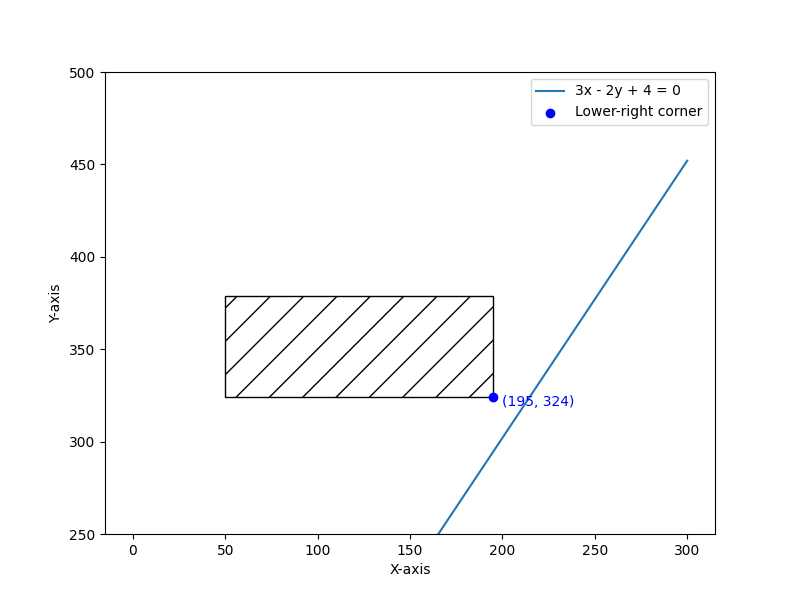
\includegraphics[width=0.5\linewidth]{figures/geometry_constraint.png}
	\caption{Geometric constraint for fixtures placement}
	\label{fig:geometricconstraint}
\end{figure}

To encode the no-overlap constraint between fixtures we employ the $\mathtt{diffn}$ global constraint~\cite{DBLP:journals/constraints/BeldiceanuCDP07}:
\begin{align*}
	\mathtt{diffn}(x, y, [\wfix_{t_i} \mid i \in [1..n]], [\hfix_{t_i} \mid i \in [1..n] ])
\end{align*}

This constraint ensures that each rectangle with origin in the lower-left corener $(x_i,y_i)$, width $\wfix_{t_i}$ and height $\hfix_{t_i}$ is not overlapping. Specifically, we use the \emph{non-strict} version of $\mathtt{diffn}$, in which zero-width rectangles can be positioned anywhere, ignoring the $\nfix{} - n$ unemployed fixtures.

The same constraint can be naturally extended to prevent fixtures from being placed within areas to be extruded, as will be described in Section~\ref{sec:second_cp_cons}.

Finally, we guarantee that the horizontal distance between two fixtures placed on different bars is at least $\wmin$. Formally, for each $i \in [1..n-1]$ we impose that:
$$x_{i} \neq x_{i+1} \implies x_{i} + \wfix_{t_{i}} + \wmin \leq x_{i+1}$$

\subsection{Objective function}
\label{sec:first_objective_function}
As illustrated in Chapter~\ref{chap:pt1_background}, is possible to maximize workpiece stability by maximizing the principal moments of inertia. Consequently, the ideal objective function would be: 

\begin{equation}
	\finer = J_\xi + J_\eta
	\label{eq:f_iner}
\end{equation}
where $J_\xi$ and $J_\eta$ are the principal moments of inertia defined in Section~\ref{sec:principal_moment_of_inertia}.

However, computing $J_\xi$ and $J_\eta$ involves nonlinear operations such as squaring, square roots, and transcendental functions (sine and cosine), which are difficult to handle efficiently with CP solvers~\cite{leyffer2009applications}.

An analysis of the moment of inertia for different fixture layouts, together with previous studies on workpiece stability~\cite{kaya2006machining,roy1999geometric,menassa1991optimization,meyer1997fixture,wallack1997planning}, indicates that workpiece stability increases when fixtures are placed far apart from one another and close to the workpiece perimeter. Based on these observations, we devised an alternative objective function, $\fdistsemi$, that maximizes the sum of the pairwise Manhattan distances between fixture centroids, augmented by the semi-perimeter of the selected fixtures.

\begin{equation}
	\fdistsemi = \sum_{1 \le i < j \le n} \left(|cx_i - cx_j| + |cy_i - cy_j|\right) + \sum_{k=1}^{n} (\wfix_{t_k} + \hfix_{t_k})
	\label{eq:f_dist_semi}
\end{equation}
\noindent where $(cx_i,cy_i) = (x_i + \frac{\wfix_{t_i}}{2}, y_i + \frac{\hfix_{t_i}}{2})$
are the coordinates of the centroid of the $i$-th placed fixture, having type $t_i$.

\section{Case study}
\label{sec:case_study}
We evaluated our approach on a real case where the workpiece is a stair step of a spiral staircase. The workpiece area, shown in Figure.~\ref{fig:stairstepworkpiece}, is defined by the following inequalities:
\begin{align*}
	(a):~ x &\geq 20 & (d):~ x &\leq 689\\
	(b):~ y &\leq 0.20x + 257.91 & (e):~ y &\geq 0.54x + -356.21\\
	(c):~ y &\leq -0.58x + 781.92 &  (f):~ y &\geq -0.20x + 139.06
\end{align*}

\begin{figure}[t]
	\centering  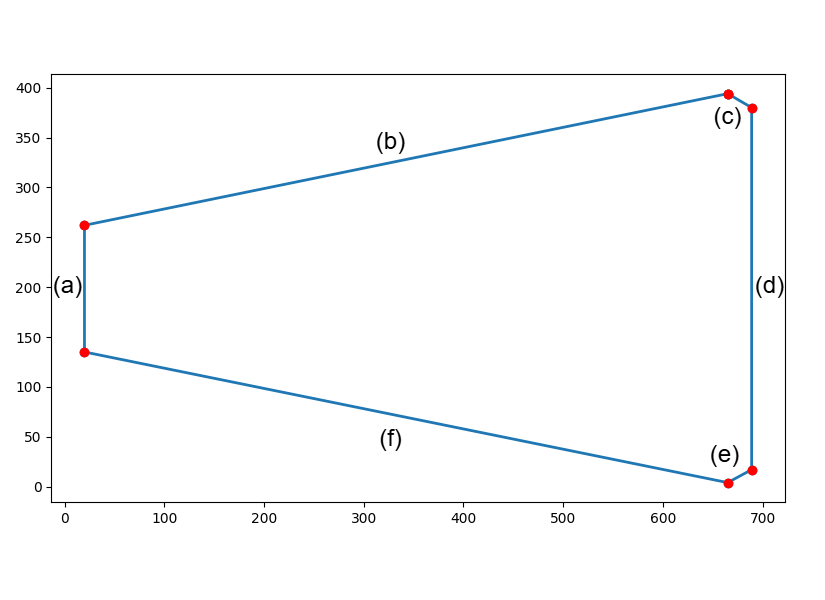
\includegraphics[width=0.5\linewidth]{figures/stair_step_line_equations.png}
	\caption{Stair step of a spiral staircase}
	\caption{A polygonal workpiece representing a stair step}
	\label{fig:stairstepworkpiece}
\end{figure}

The width and height of the worktable are respectively $\wtab = 700$ and $\htab = 400$.
The minimal horizontal distance between fixtures is $\wmin = 140$.
We have two different types of fixtures available:
\begin{itemize}
	\item five square fixtures of dimension \(145 \times 145 \text{ mm}\);
	\item five rectangular fixtures of dimension \(145 \times 55 \text{ mm}\).
\end{itemize}
So, $\nfix_{1} = \nfix_{2} = 5$ with $\wfix_{1} = \hfix_{1} = \wfix_{2} = 145$ and $\hfix_{2}=55$.

We set an upper bound $\nmax$ on the number of fixtures (i.e., we impose $n\leq\nmax$) and we evaluated different values of $\nmax$ in the range $[2..10]$.
We assume a minimum number of 2 fixtures (i.e., $n \geq 2$) as placing only one fixture is not a realistic case.

We defined two models, one using the objective function $\finer$ and the other using $\fdistsemi$. Both were implemented in Minizinc~\cite{nethercote2007minizinc}. For the model using $\fdistsemi$, four solvers were evaluated: Chuffed~\cite{chuffed}, Gecode~\cite{schulte2006gecode}, OR-Tools~\cite{ortools} and Gurobi~\cite{gurobi}. For the $\finer$ model, we restricted our evaluation to solvers that support floating-point variables, namely Gecode and Gurobi.

All experiments were conducted with a time limit of 300 seconds on a 64-bit Windows machine equipped with an Intel Core i5 CPU and 16 GB of RAM. 

Table~\ref{tab:solvercomparison_momentobj} and Table~\ref{tab:solvercomparison_distobj} report the results obtained using $\finer$ and $\fdistsemi$ as objective functions, respectively, across different values of $\nmax$. Specifically, Table~\ref{tab:solvercomparison_distobj} doesn't report the value of $\fdistsemi$ but the corresponding \emph{a posteriori} values of $\finer$ for the best solutions found by the solvers.

In Table~\ref{tab:solvercomparison_momentobj} the result for the Gecode solver are not reported, as it fails to find any feasible solution within the time limit. On the other hand, Gurobi being a MIP solver that handle continuous variables, is able to find optimal solutions for $\nmax \leq 5$ but is not able to find any solution for $\nmax \geq 6$. 

When using $\fdistsemi$ as the objective function, Table~\ref{tab:solvercomparison_distobj} shows that all solvers are able to find at least one feasible solution for every value of $\nmax$, with Chuffed and Gurobi solving all instances to optimality. Overall, the best performance is achieved by Chuffed, which is able to reach the optimal solutions in less time than Gurobi.

In the tables the optimal solutions found are reported in bold, the $\fdistsemi$ objective function can admit multiple equivalent optimal solutions; however, these solutions may lead to different values of $\finer$, due to the high sensitivity of the moments of inertia to small fixture displacements, as reported for $\nmax \in {3,4,5}$ in Table~\ref{tab:solvercomparison_distobj}.

Comparing the two tables, we can observe that solutions generated using $\fdistsemi$ generally achieve lower $\finer$ values, but can be computed significantly faster, making this objective function particularly suitable for large workpieces or instances requiring a high number of fixtures. Indeed, comparing the runtimes obtained by Gurobi with the two objective functions shows that solving the problem with $\fdistsemi$ is on average more than 150 times faster than using $\finer$.

\begin{landscape}
	
	\begin{table}[p]
		\centering
		\small
		\caption{Results for $\finer$. All $\finer$ values reported in units of $10^9$. Bold fold indicates the best $\finer$ value found before the timeout.}
		\label{tab:solvercomparison_momentobj}
		\renewcommand{\arraystretch}{1.2}
		
		\begin{tabular}{p{1.5cm}p{1.5cm}ccccccccc}
			\toprule
			\multicolumn{2}{c}{} & \multicolumn{9}{c}{$\nmax$} \\
			\cmidrule(lr){3-11}
			\textbf{Solver} & \textbf{Metric} & 2 & 3 & 4 & 5 & 6 & 7 & 8 & 9 & 10 \\
			\midrule
			Gurobi & Runtime [ms]
			& 14250 & 189000 & 90000 & 258000 & -- & -- & -- & -- & -- \\
			& $\finer$
			& \textbf{2.65072}
			& \textbf{3.79990}
			& \textbf{3.79990}
			& \textbf{3.87506}
			& 3.89034
			& --
			& --
			& --
			& -- \\
			\bottomrule
		\end{tabular}
	\end{table}
	
\end{landscape}

\begin{landscape}
	
	\begin{table}[p]
		\centering
		\small
		\caption{Results using $\fdistsemi$. Bold fold denotes the $\finer$, reported in units of $10^9$, corresponding to a $\fdistsemi$-optimal solution.}
		\label{tab:solvercomparison_distobj}
		\renewcommand{\arraystretch}{1.0}
		
		\begin{tabular}{p{1.5cm}p{1.5cm}ccccccccc}
			\toprule
			\multicolumn{2}{c}{} & \multicolumn{9}{c}{$\nmax$} \\
			\cmidrule(lr){3-11}
			\textbf{Solver} & \textbf{Metric} & 2 & 3 & 4 & 5 & 6 & 7 & 8 & 9 & 10 \\
			\midrule
			
			Chuffed & Runtime [ms]
			& 1566 & 904 & 2039 & 3333 & 3700 & 2533 & 4873 & 5222 & 5593 \\
			& $\finer$
			& \textbf{2.64416}
			& \textbf{2.38480}
			& \textbf{2.58584}
			& \textbf{3.54968}
			& \textbf{3.80905}
			& \textbf{3.80905}
			& \textbf{3.80905}
			& \textbf{3.80905}
			& \textbf{3.80905} \\
			\midrule
			
			Gurobi & Runtime [ms]
			& 503 & 745 & 961 & 1098 & 1540 & 1856 & 4674 & 5534 & 10840 \\
			& $\finer$
			& \textbf{2.64416}
			& \textbf{2.38350}
			& \textbf{2.58584}
			& \textbf{3.08459}
			& \textbf{3.80905}
			& \textbf{3.80905}
			& \textbf{3.80905}
			& \textbf{3.80905}
			& \textbf{3.80905} \\
			\midrule
			
			Gecode & Runtime [ms]
			& 549 & 18292 & -- & -- & -- & -- & -- & -- & -- \\
			& $\finer$
			& \textbf{2.64416}
			& \textbf{2.39170}
			& 2.58584
			& 2.58584
			& 2.58584
			& 3.73308
			& 2.58584
			& 2.58584
			& 2.58584 \\
			\midrule
			
			OR-Tools & Runtime [ms]
			& 882 & 7804 & 260000 & -- & -- & -- & -- & -- & -- \\
			& $\finer$
			& \textbf{2.64416}
			& \textbf{2.16912}
			& \textbf{2.24606}
			& \textbf{3.34565}
			& 3.34565
			& 3.38321
			& 3.73467
			& 3.73467
			& 3.67863 \\
			\bottomrule
		\end{tabular}
		
	\end{table}
	
\end{landscape}

Tables~\ref{tab:visual_results_234_fdist} and~\ref{tab:visual_results_5_10_fdist} present the visual results obtained from the different solvers using the $\fdistsemi$ objective function, evaluated across varying values of $\nmax$, while Tables~\ref{tab:visual_results_234_finer} and~\ref{tab:visual_results_5_10_finer} report the corresponding layouts obtained with Gurobi when optimizing $\finer$.

The layouts obtained with $\fdistsemi$ are generally similar across solvers. However, when the number of fixtures is limited to three, Chuffed, Gecode, and OR-Tools tend to place a smaller fixture on the left side of the workpiece, below its center, whereas Gurobi positions the smaller fixture closer to the center and places two larger fixtures on the right side, leading to a higher $\finer$ value, as reported in Table~\ref{tab:solvercomparison_distobj}.

As expected, optimizing $\finer$ promotes the selection of larger fixtures, since larger support areas result in higher moments of inertia. For instance, with three fixtures, the solution provided by Gurobi using the $\finer$ objective function selects only the largest available fixtures. This configuration is maintained also for $\nmax=4$, where the solver avoids introducing an additional fixture.


\begin{landscape}
	
	% =====================================================
	% TABLE 1: n = 2–4 (all solvers EXCEPT Gurobi f_iner)
	% =====================================================
	\begin{table}[p]
		\centering
		\small
		\caption{Visual results for solvers’ solutions using $\fdistsemi$ as objective function ($\nmax = 2$--$4$).}
		\label{tab:visual_results_234_fdist}
		\renewcommand{\arraystretch}{1.5}
		
		\begin{tabular}{lccc}
			\toprule
			\multicolumn{1}{c}{} & \multicolumn{3}{c}{$\nmax$} \\
			\cmidrule(lr){2-4}
			\textbf{Solver} & 2 & 3 & 4 \\
			\midrule
			
			\raisebox{+6.0\height}{Chuffed} &
			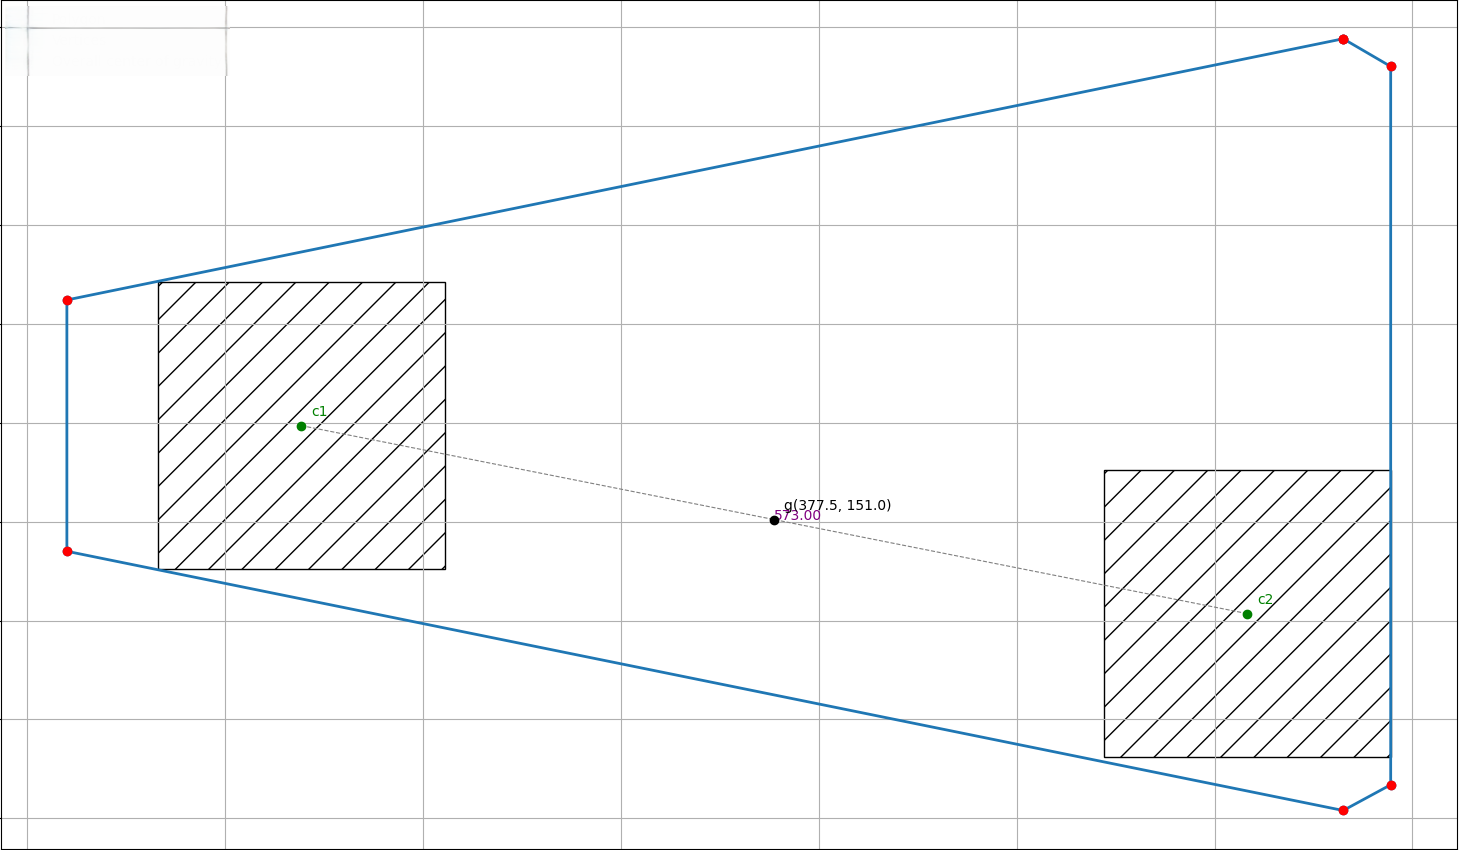
\includegraphics[width=1.8in]{figures/chuffed2.png} &
			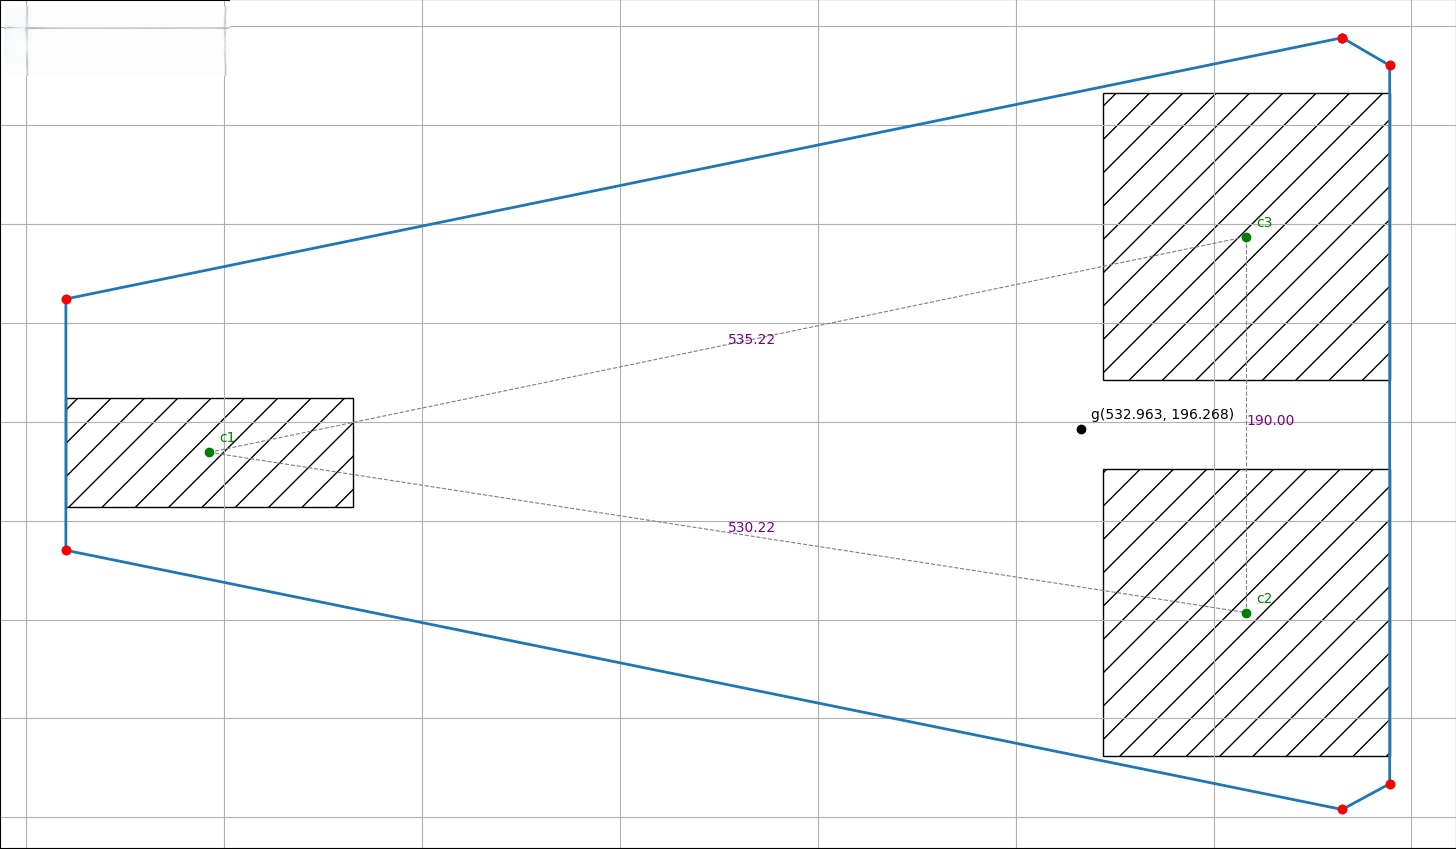
\includegraphics[width=1.8in]{figures/chuffed3.png} &
			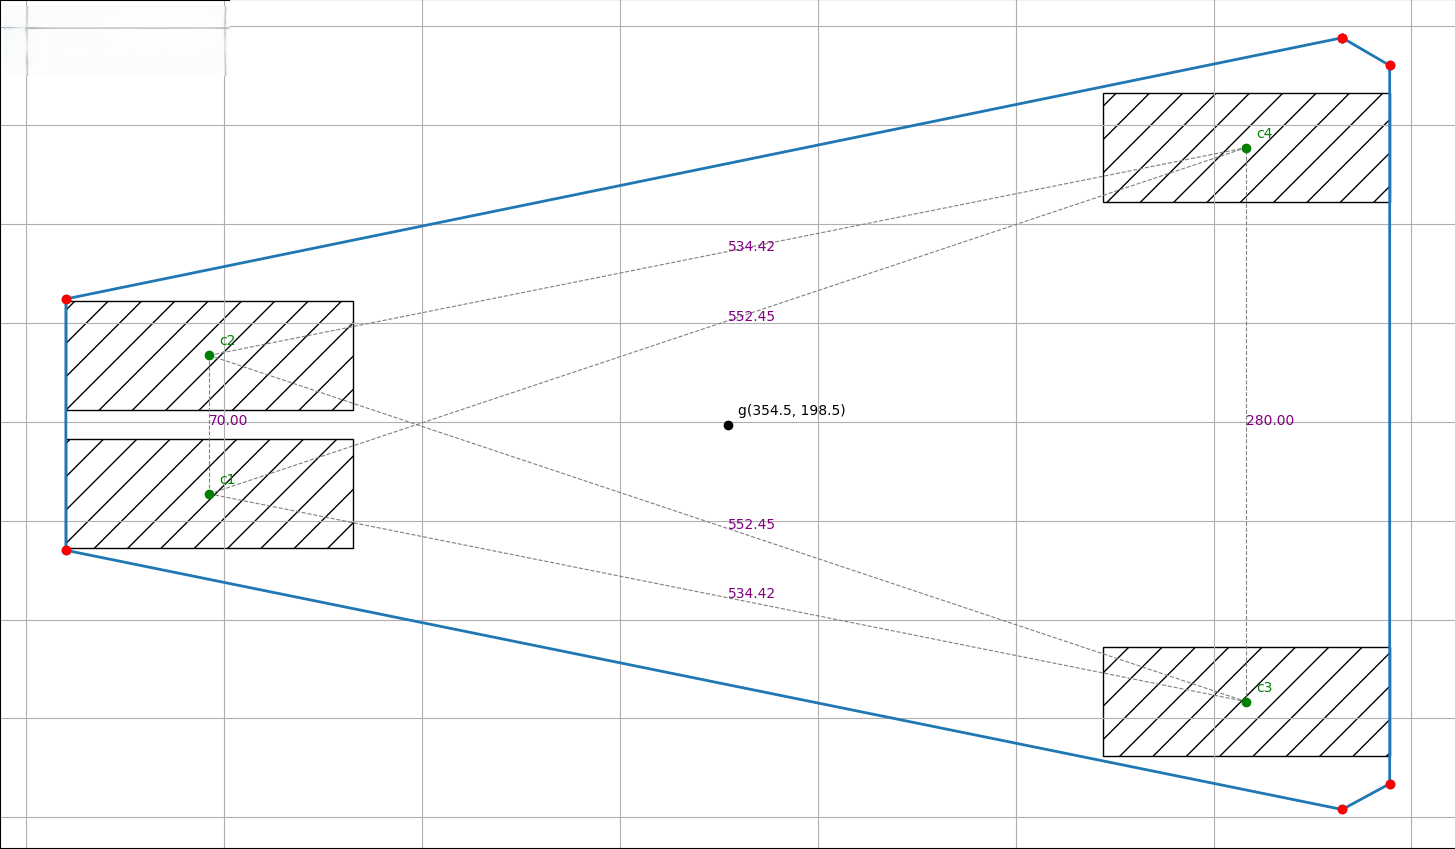
\includegraphics[width=1.8in]{figures/chuffed4.png} \\
			
			\raisebox{+6.0\height}{Gecode ($\fdistsemi$)} &
			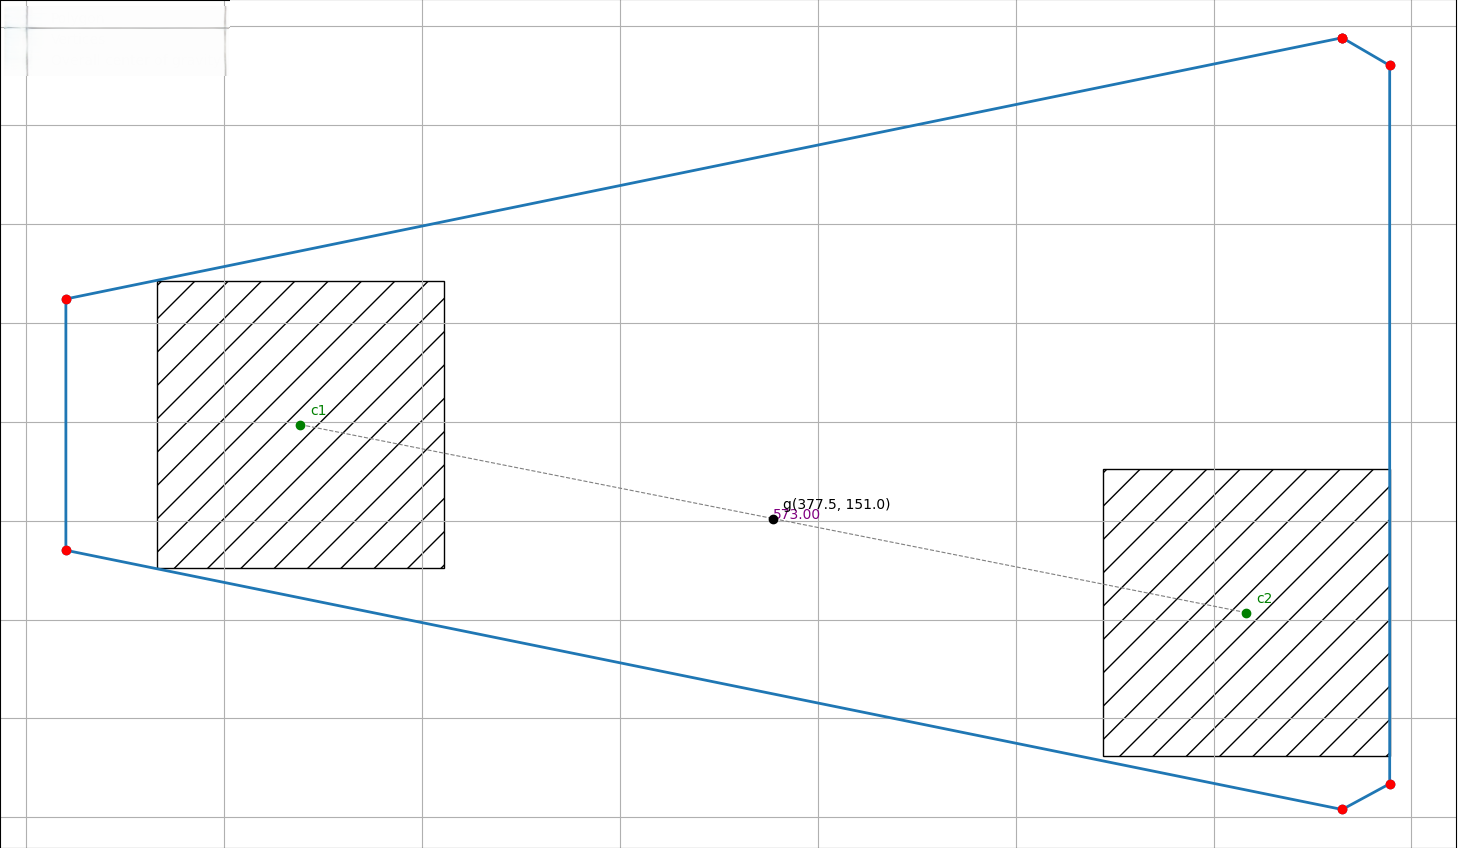
\includegraphics[width=1.8in]{figures/gecode2.png} &
			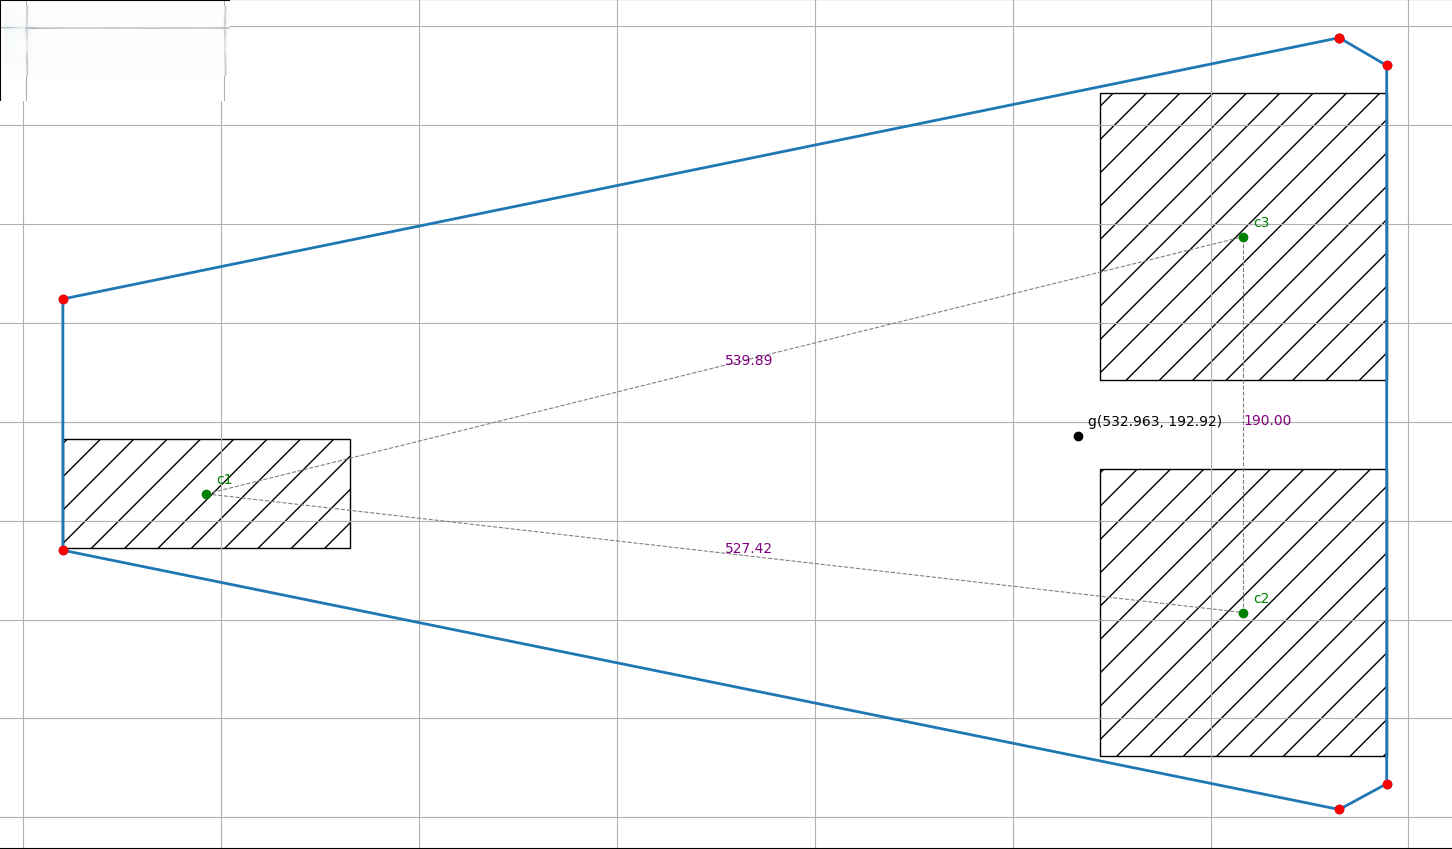
\includegraphics[width=1.8in]{figures/gecode3.png} &
			\raisebox{+12.0\height}{--} \\
			
			\raisebox{+6.0\height}{OR-Tools} &
			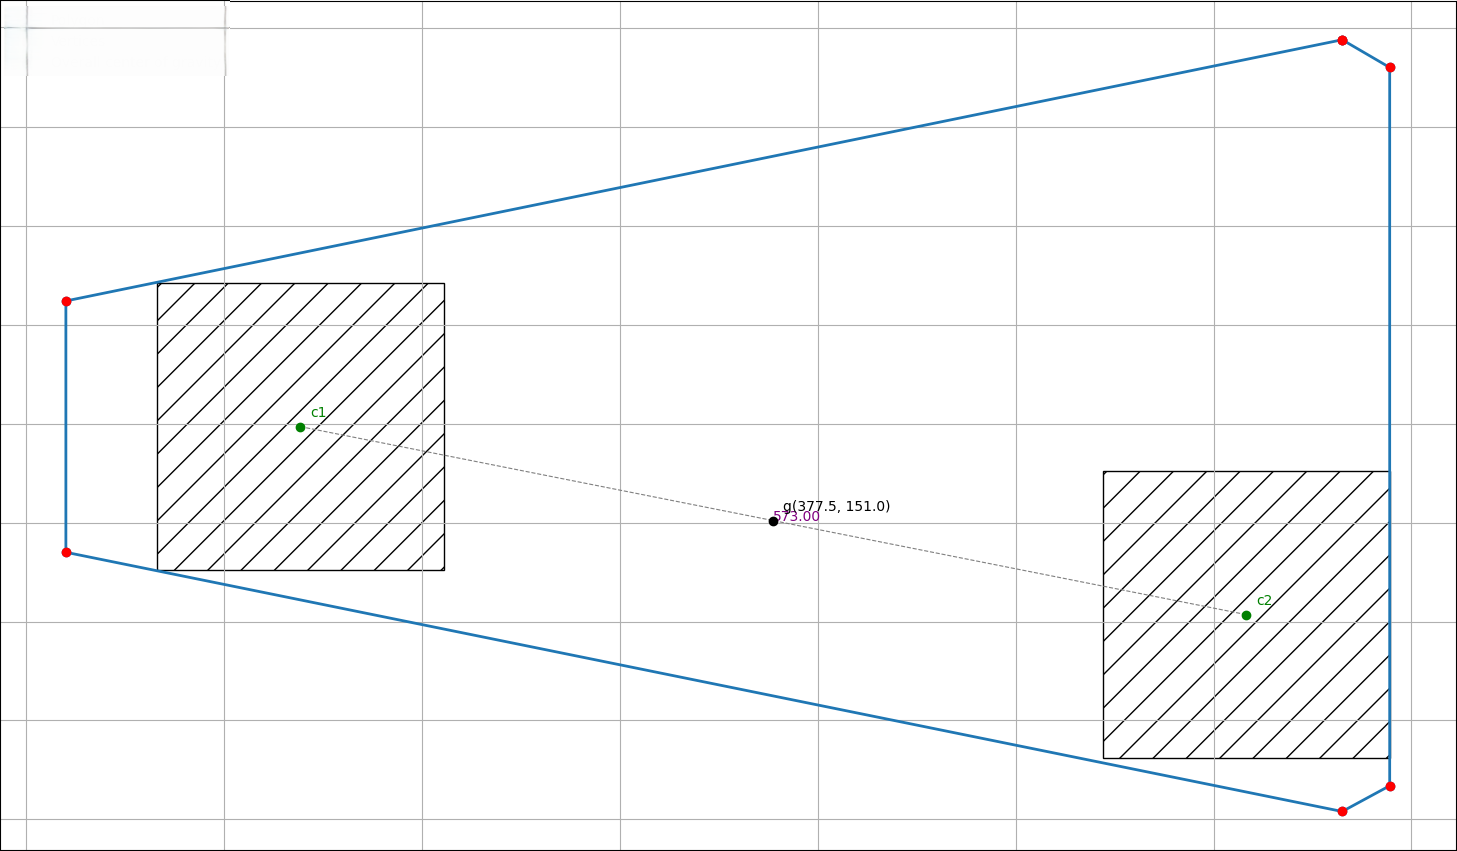
\includegraphics[width=1.8in]{figures/ortools2.png} &
			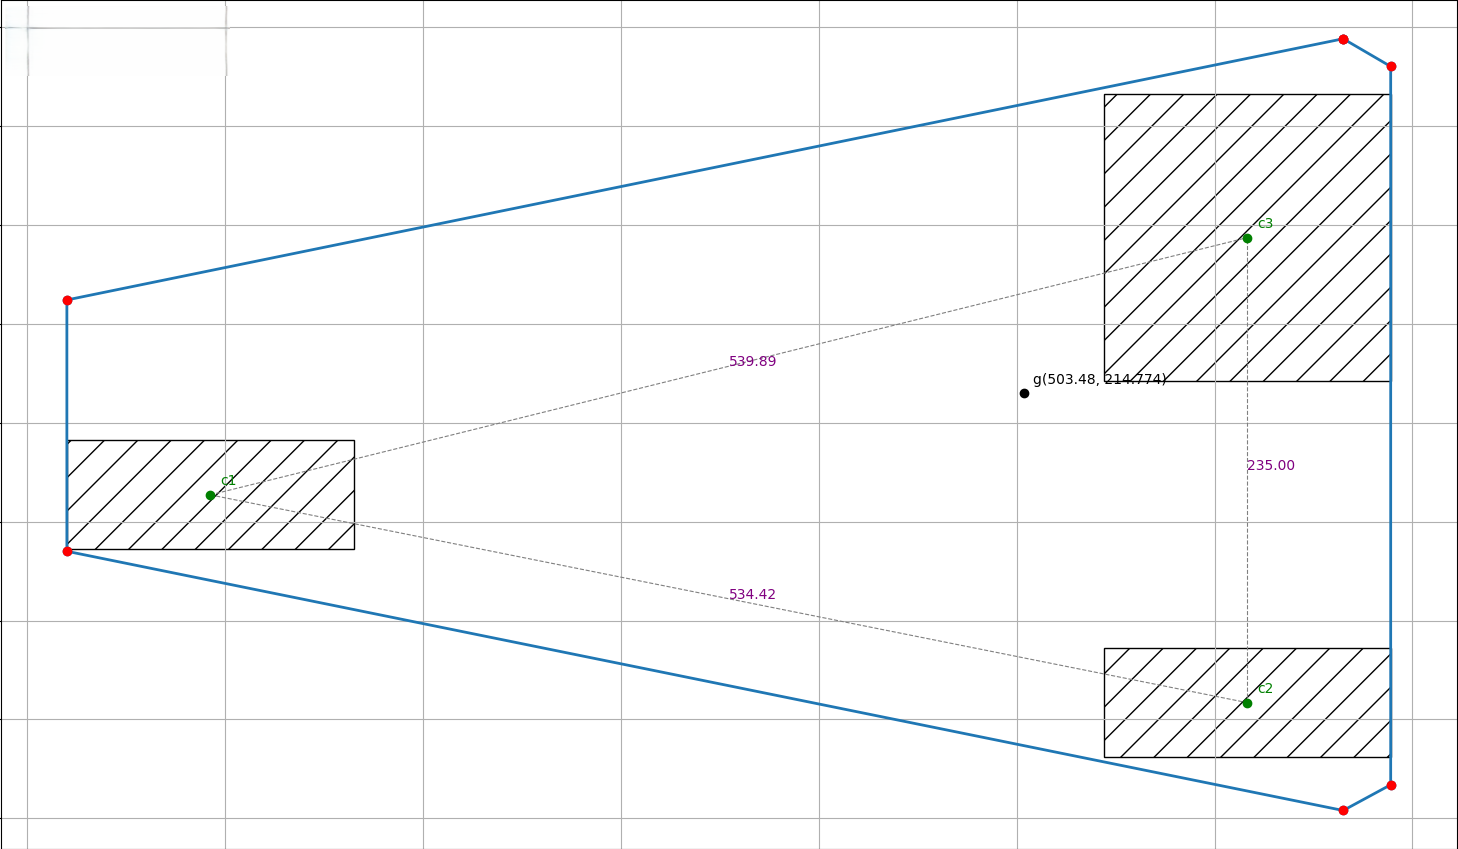
\includegraphics[width=1.8in]{figures/ortools3.png} &
			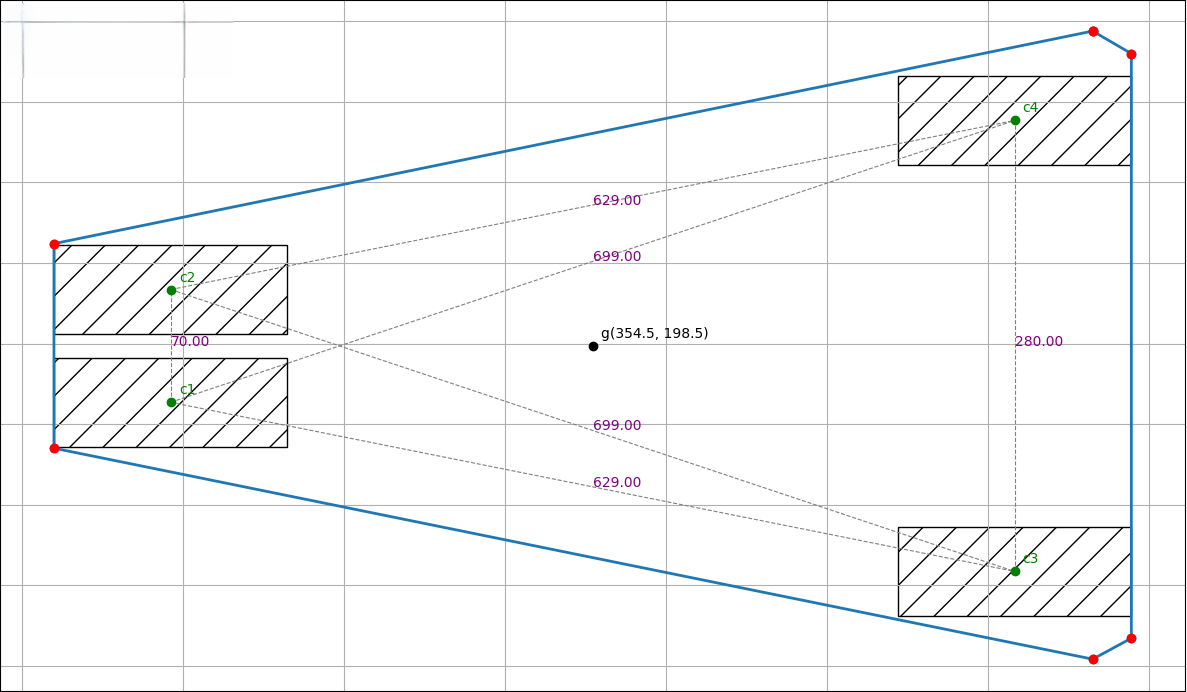
\includegraphics[width=1.8in]{figures/ortools4.png} \\
			
			\raisebox{+6.0\height}{Gurobi ($\fdistsemi$)} &
			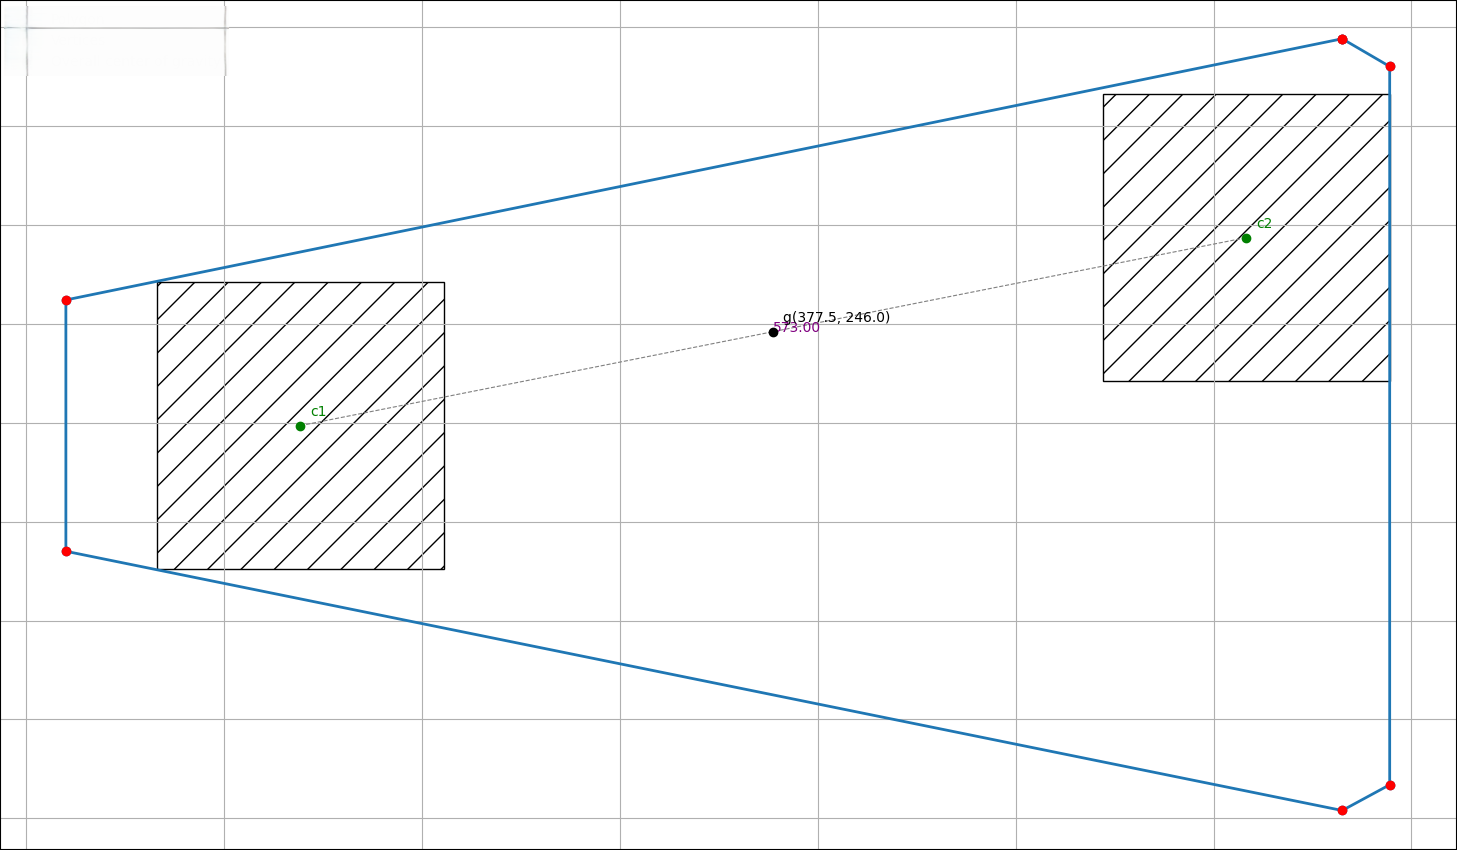
\includegraphics[width=1.8in]{figures/gurobi2.png} &
			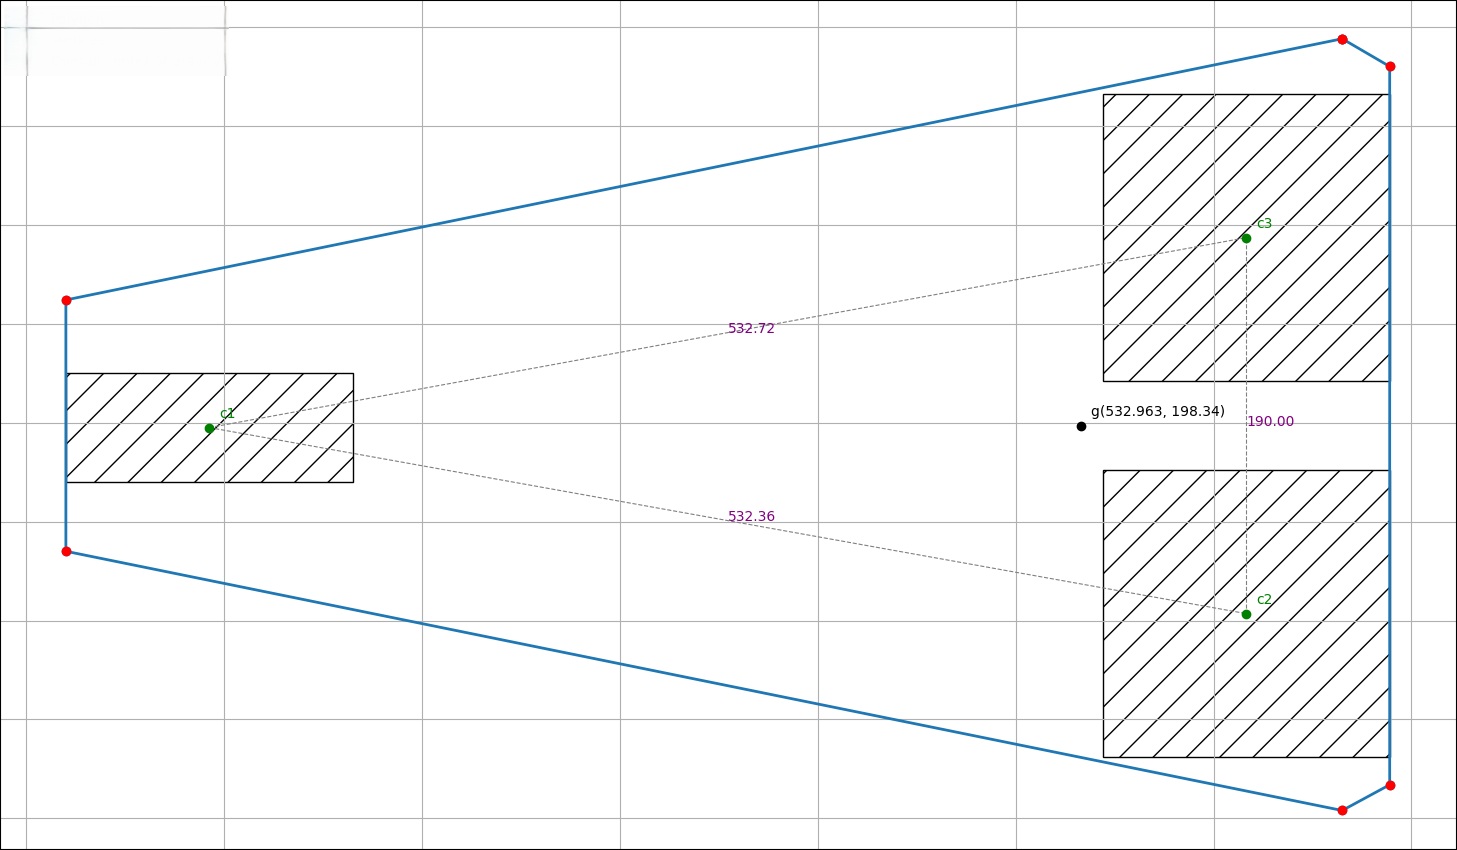
\includegraphics[width=1.8in]{figures/gurobi3.png} &
			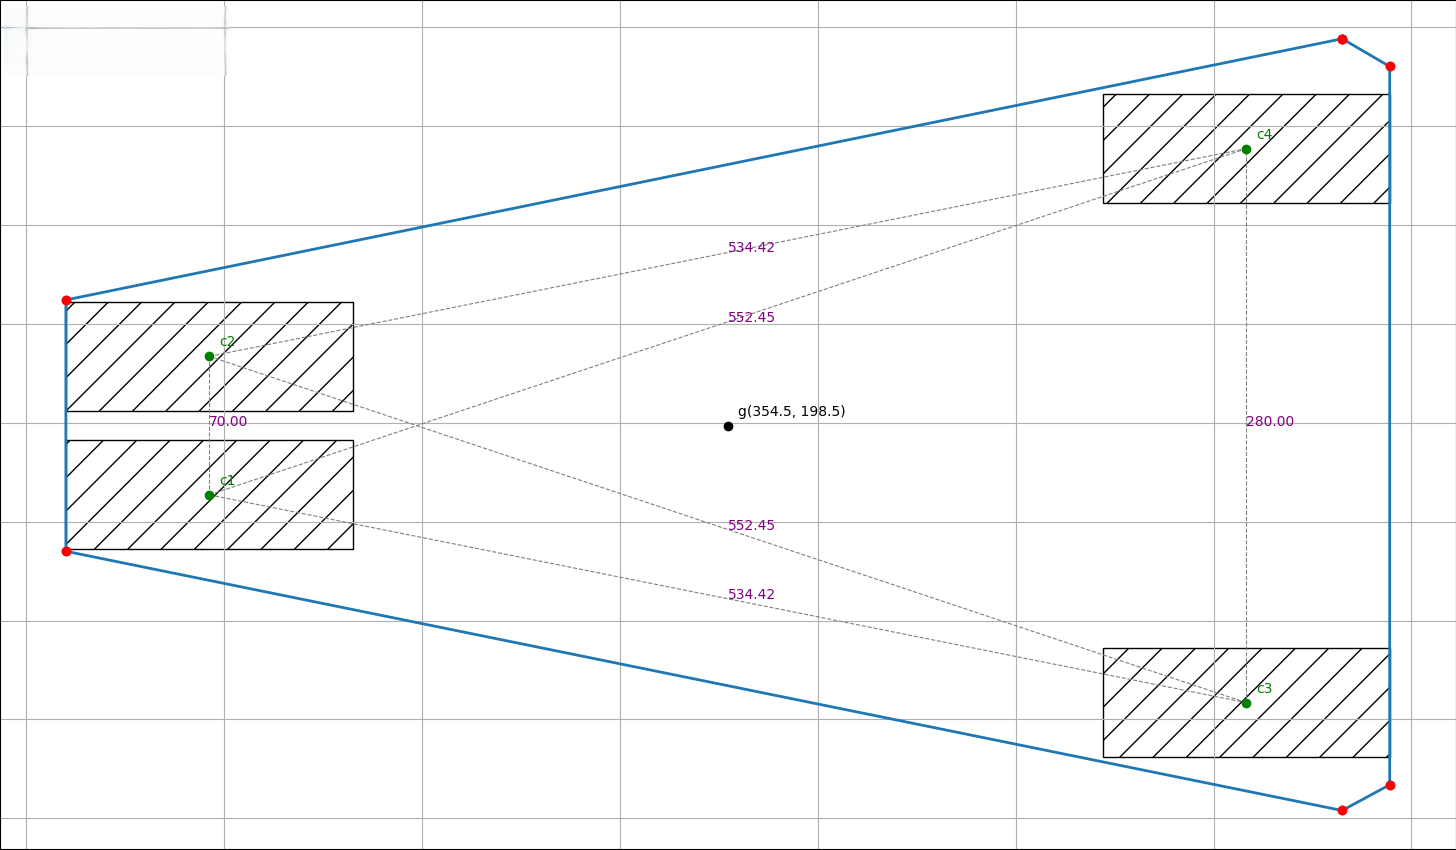
\includegraphics[width=1.8in]{figures/gurobi4.png} \\
			
			\bottomrule
		\end{tabular}
	\end{table}
	
	% =====================================================
	% TABLE 3: n = 5–10 (all solvers EXCEPT Gurobi f_iner)
	% =====================================================
	\begin{table}[p]
		\centering
		\small
		\caption{Visual results for solvers’ solutions using $\fdistsemi$ objective function ($\nmax = 5$--$10$).}
		\label{tab:visual_results_5_10_fdist}
		\renewcommand{\arraystretch}{1.5}
		
		\begin{tabular}{lcc}
			\toprule
			\multicolumn{1}{c}{} & \multicolumn{2}{c}{$\nmax$} \\
			\cmidrule(lr){2-3}
			\textbf{Solver} & 5 & 6--10 \\
			\midrule
			
			\raisebox{+6.0\height}{Chuffed} &
			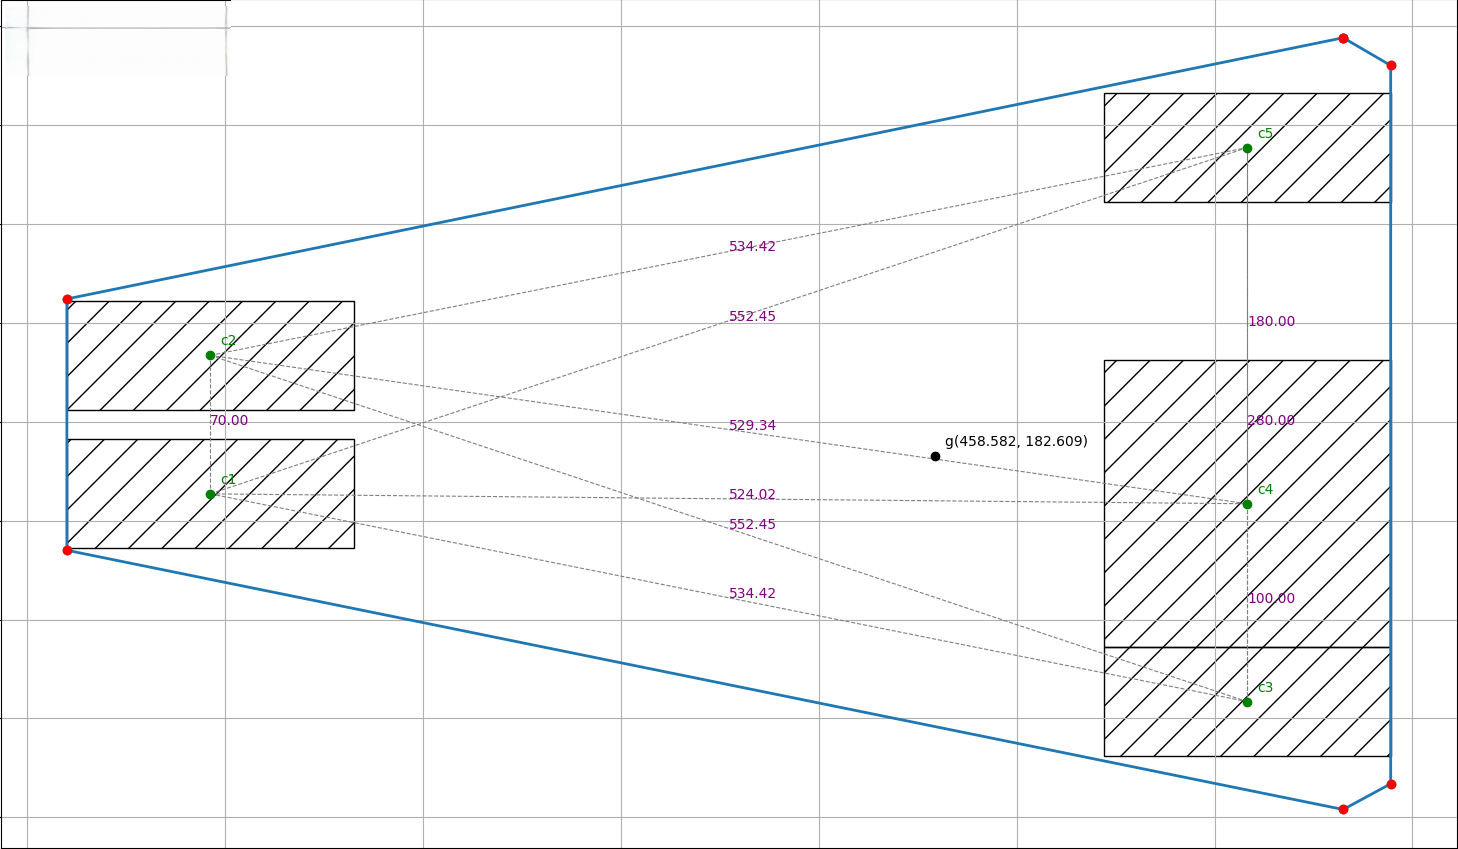
\includegraphics[width=1.8in]{figures/chuffed5.png} &
			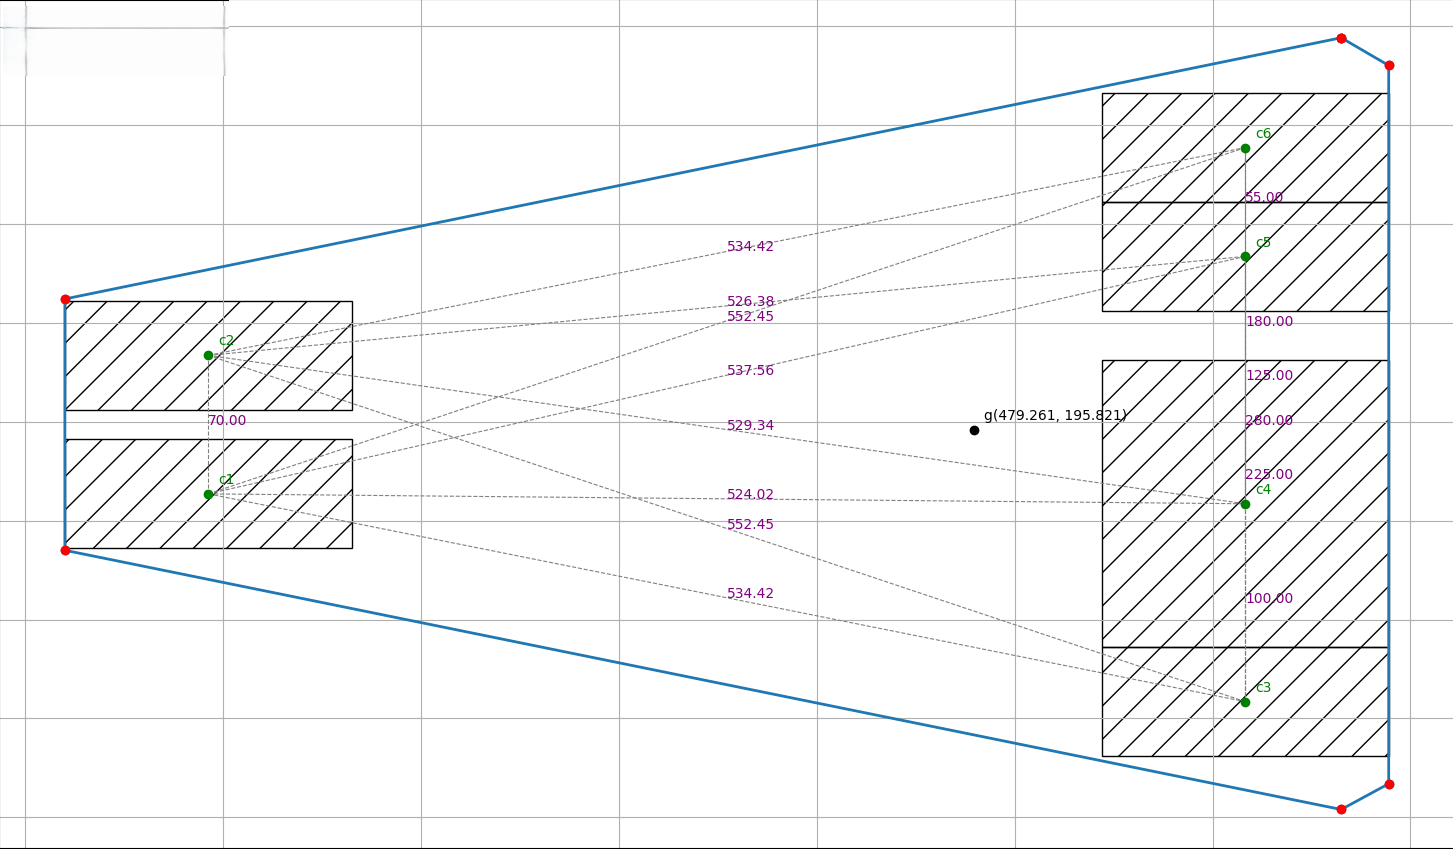
\includegraphics[width=1.8in]{figures/chuffed6.png} \\
			
			\raisebox{+6.0\height}{OR-Tools} &
			\raisebox{+12.0\height}{--} &
			\raisebox{+12.0\height}{--} \\
			
			\raisebox{+6.0\height}{Gurobi ($\fdistsemi$)} &
			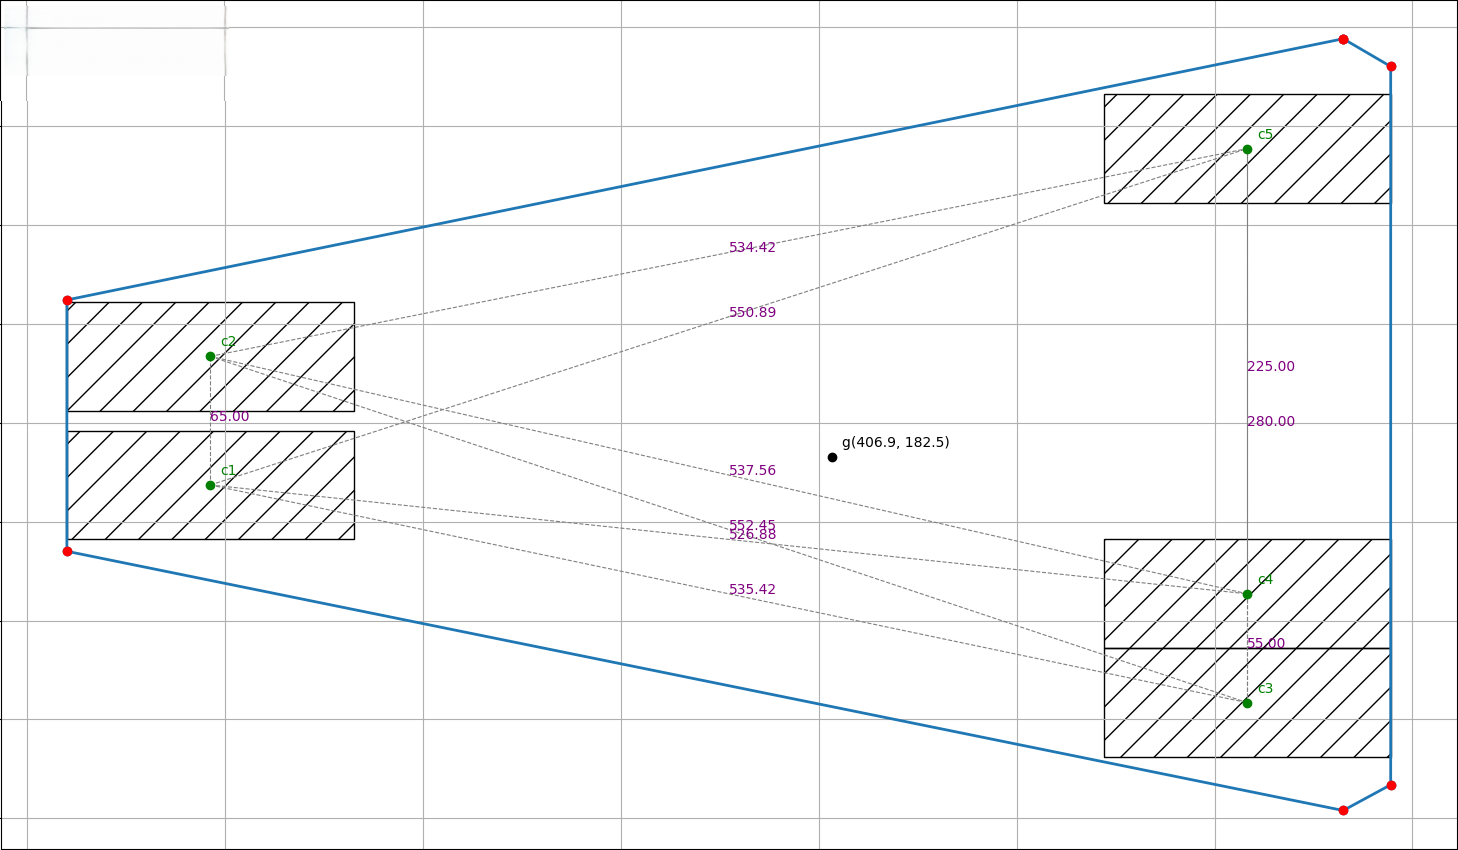
\includegraphics[width=1.8in]{figures/gurobi5.png} &
			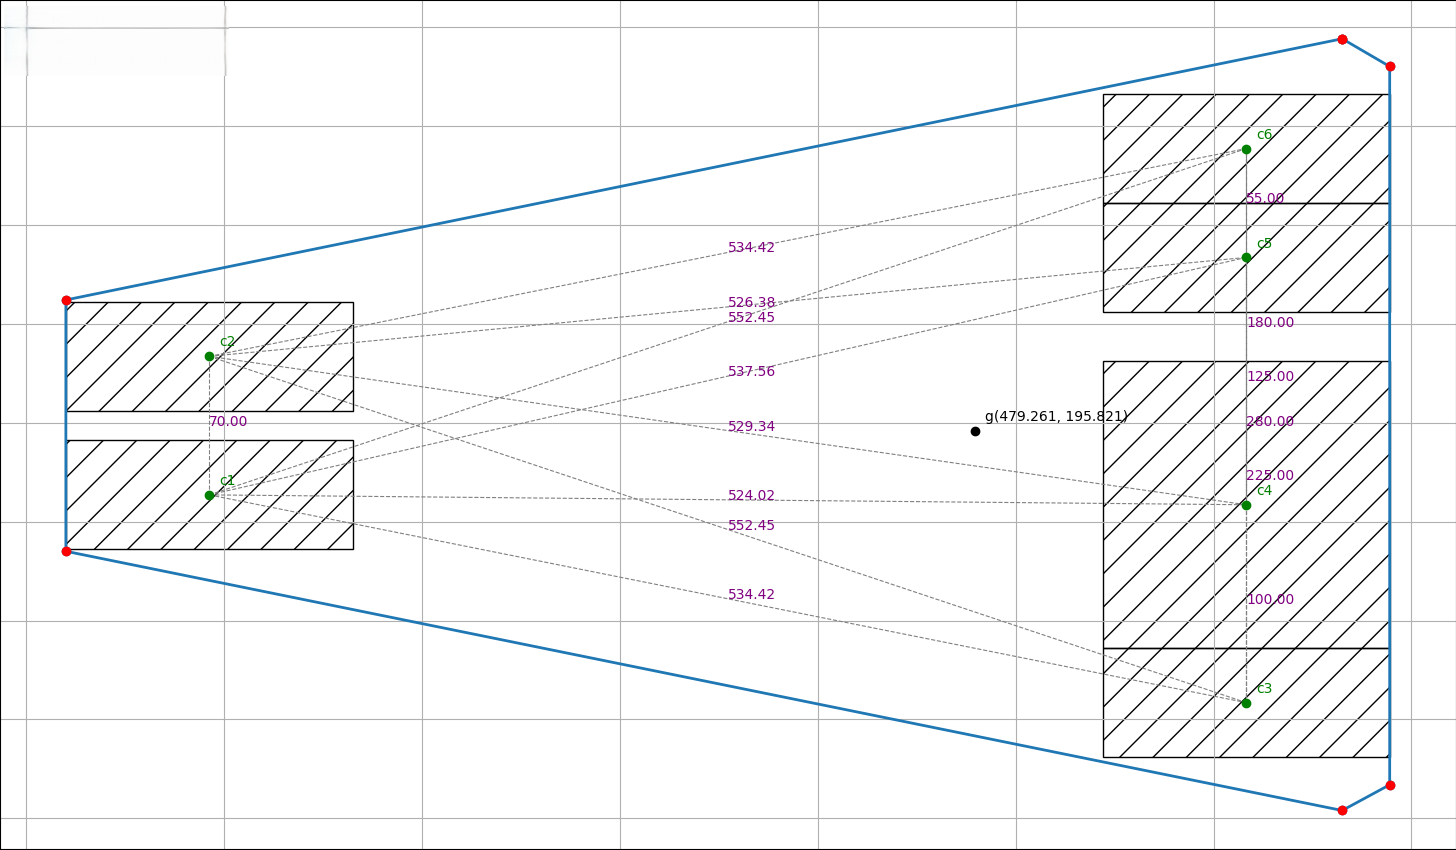
\includegraphics[width=1.8in]{figures/gurobi6.png} \\
			
			\bottomrule
		\end{tabular}
	\end{table}
	
		% =====================================================
	% TABLE 2: n = 2–4 (Gurobi f_iner ONLY)
	% =====================================================
	\begin{table}[p]
		\centering
		\small
		\caption{Visual results for Guorbi solver solutions using $\finer$ objective function ($\nmax = 2$--$4$).}
		\label{tab:visual_results_234_finer}
		\renewcommand{\arraystretch}{1.5}
		
		\begin{tabular}{lccc}
			\toprule
			\multicolumn{1}{c}{} & \multicolumn{3}{c}{$\nmax$} \\
			\cmidrule(lr){2-4}
			\textbf{Solver} & 2 & 3 & 4 \\
			\midrule
			
			Gurobi ($\finer$) &
			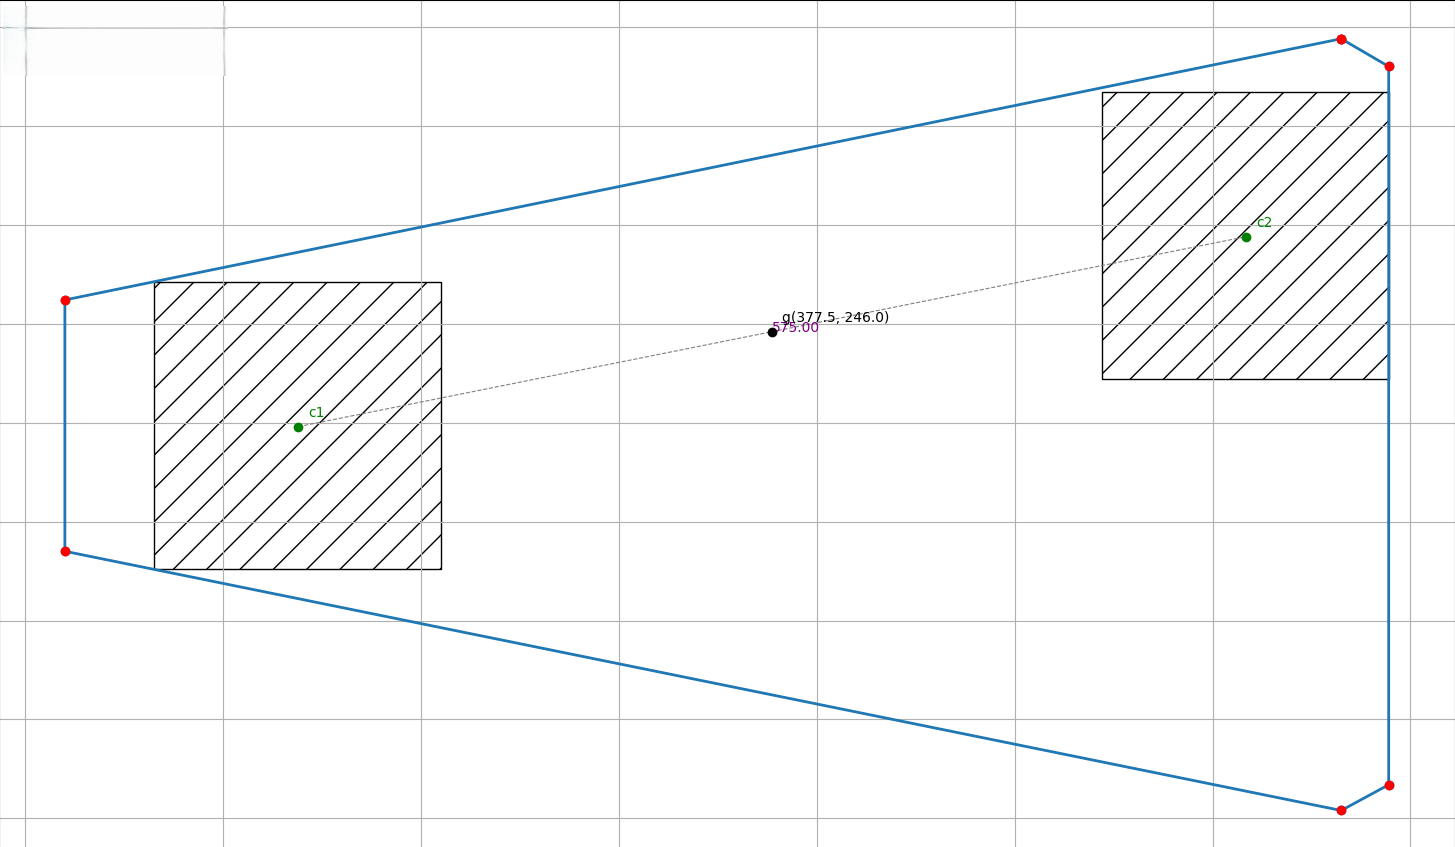
\includegraphics[width=1.8in]{figures/gurobi2_moments.png} &
			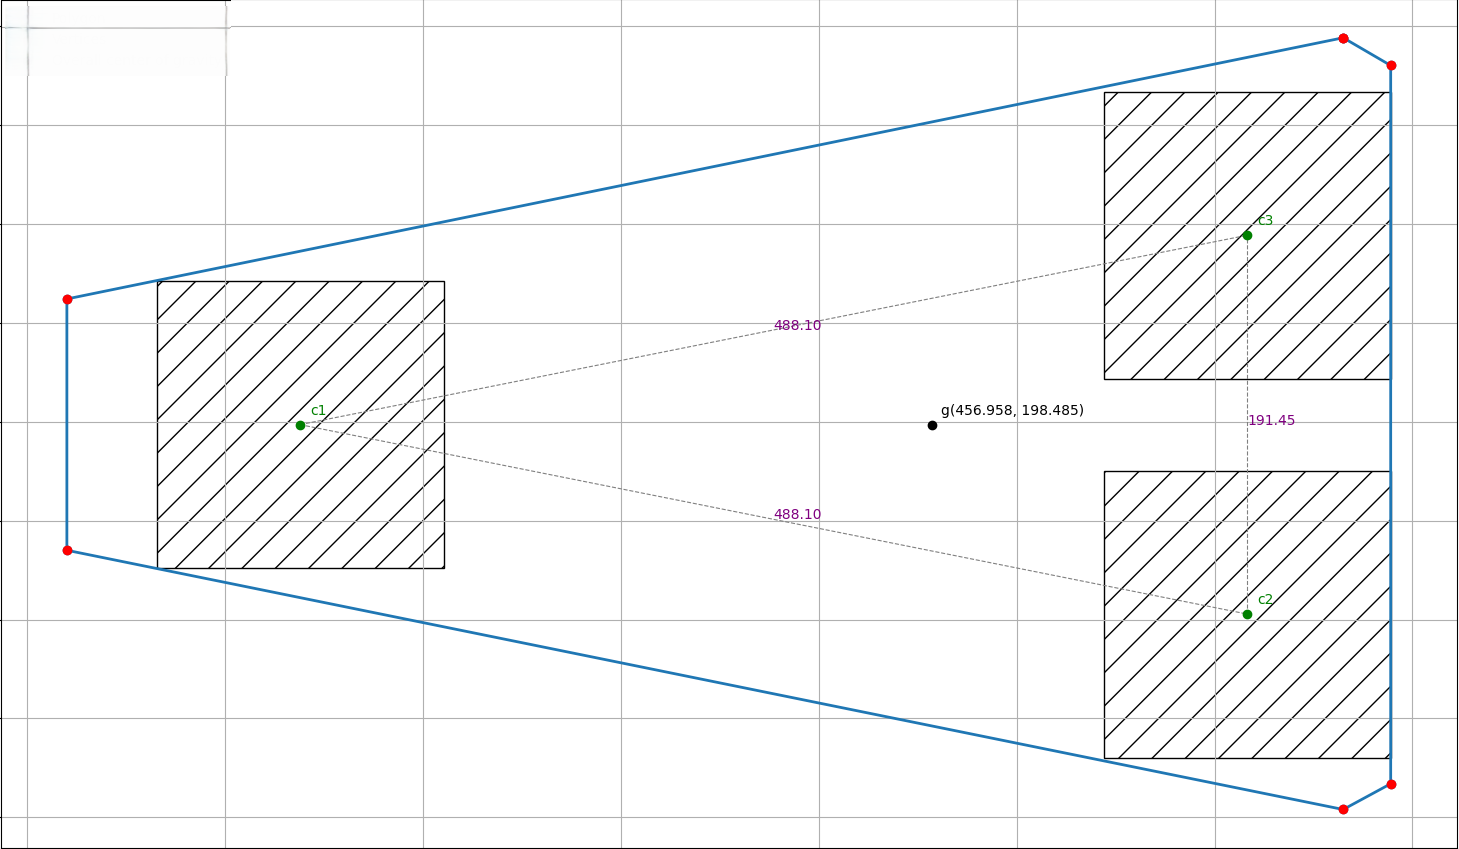
\includegraphics[width=1.8in]{figures/gurobi3_moments.png} &
			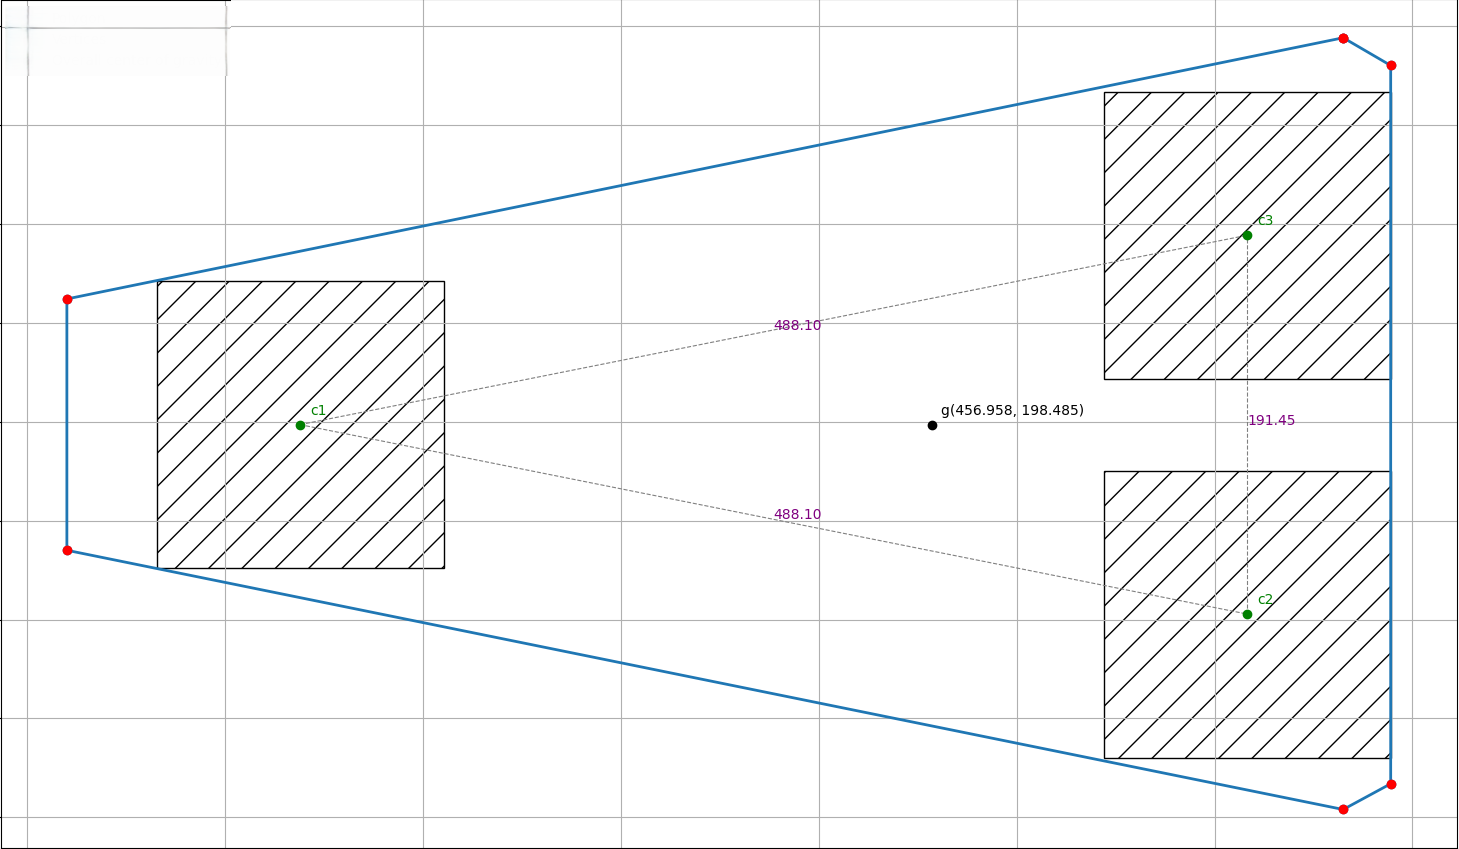
\includegraphics[width=1.8in]{figures/gurobi3_moments.png} \\
			
			\bottomrule
		\end{tabular}
	\end{table}
	
	% =====================================================
	% TABLE 4: n = 5–10 (Gurobi f_iner ONLY)
	% =====================================================
	\begin{table}[p]
		\centering
		\small
		\caption{Visual results for Guorbi solver solutions using $\finer$ objective function ($\nmax = 5$--$10$).}
		\label{tab:visual_results_5_10_finer}
		\renewcommand{\arraystretch}{1.5}
		
		\begin{tabular}{lcc}
			\toprule
			\multicolumn{1}{c}{} & \multicolumn{2}{c}{$\nmax$} \\
			\cmidrule(lr){2-3}
			\textbf{Solver} & 5 & 6--10 \\
			\midrule
			
			Gurobi ($\finer$) &
			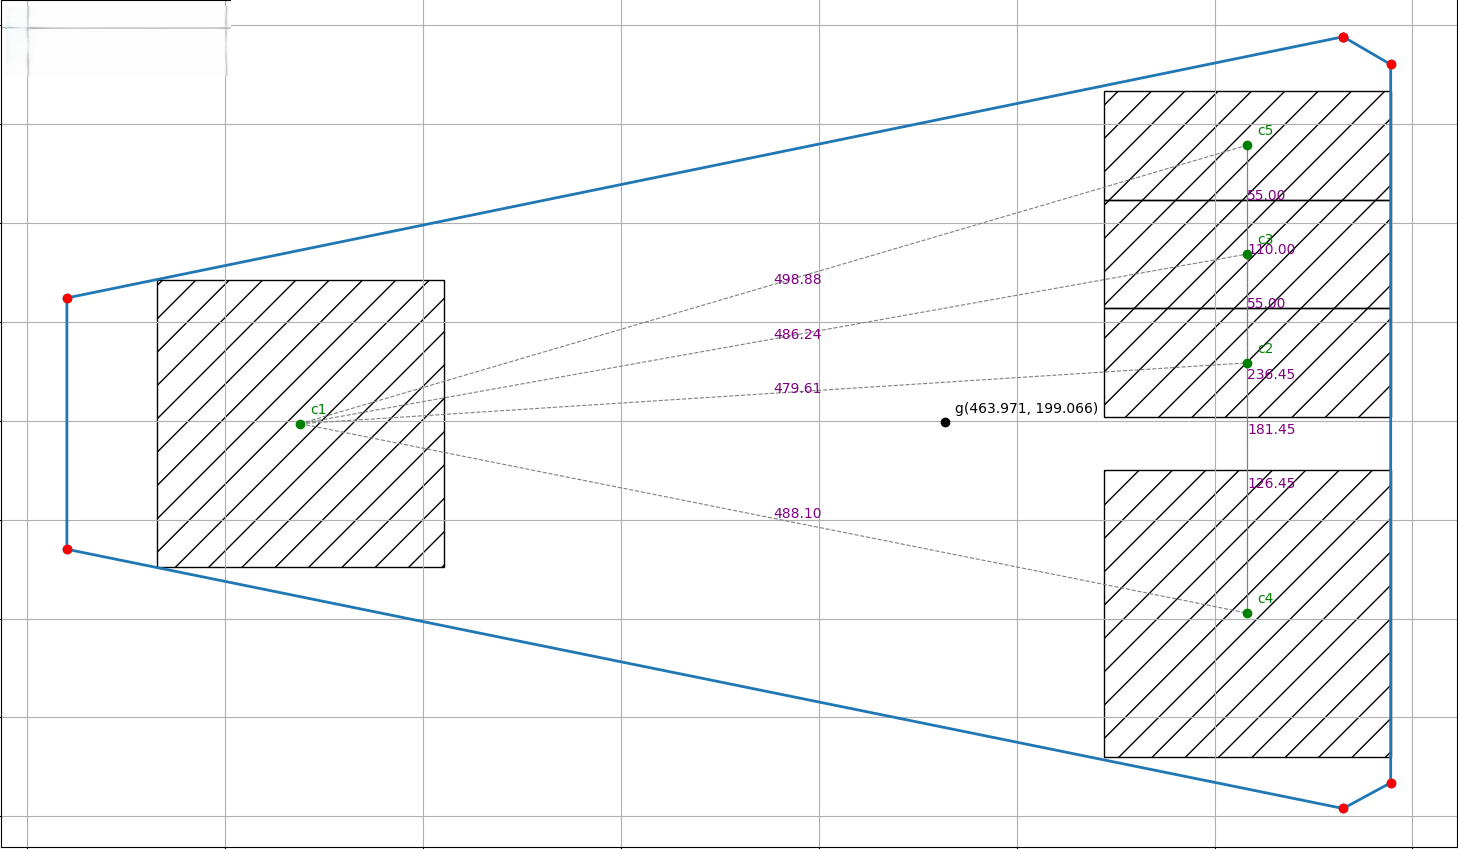
\includegraphics[width=1.8in]{figures/gurobi5_moments.png} &
			\raisebox{+12.0\height}{--} \\
			
			\bottomrule
		\end{tabular}
	\end{table}
	
	
	
\end{landscape}